\documentclass{article}
\usepackage{amsmath}
\usepackage{amssymb}
\usepackage{graphicx}
\usepackage{tikz}
\usepackage{pgfplots}
\usepackage{float}
\usepackage{subcaption}
\usepackage{geometry}

\geometry{a4paper, margin=1in}

% Define example environment
\newenvironment{example}[1]{
    \begin{trivlist}
    \item[\textbf{Example:}] #1
    \vspace{0.5em}
}{
    \end{trivlist}
    \vspace{1em}
}

\pgfplotsset{compat=1.18}
\usetikzlibrary{patterns,decorations.pathreplacing}

\title{Lecture 5 Examples}
\author{Signals and Systems Course}
\date{}

\begin{document}

\maketitle

\begin{example}[1. Continuous-Time Convolution: Exponential and Unit Step]
\textbf{Problem:}
Find the convolution $y(t) = x(t) * h(t)$ where:
\begin{align}
    x(t) &= u(t) \quad \text{(unit step function)} \\
    h(t) &= e^{-at} u(t), \quad a > 0 \quad \text{(exponential impulse response)}
\end{align}

\begin{figure}[H]
    \centering
    \begin{minipage}{0.45\textwidth}
        \centering
        \resizebox{!}{5cm}{ \begin{tikzpicture}
	\begin{axis}[
		width=12cm,
		height=7cm,
		title={Unit Step Function $x(t) = u(t) = 
			\begin{cases} 
				1, & t \ge 0 \\
				0, & t < 0
			\end{cases}$
		},
		xlabel={$t$},
		ylabel={$x(t)$},
		axis lines=middle,
		xmin=-1.5, xmax=4.5,
		ymin=0, ymax=1.5,
		xtick={-1, 1, 2, 3, 4},
		ytick={1},
		grid=major,
		grid style={line width=.1pt, draw=gray!30},
		]
		
		% Draw the two parts of the function
		\draw[blue, very thick] (axis cs:-1.5, 0) -- (axis cs:0, 0);
		\draw[blue, very thick] (axis cs:0, 1) -- (axis cs:4.5, 1);
		
		% Mark the discontinuity at t=0
		\addplot[only marks, blue, mark=*, mark size=2pt] coordinates {(0,1)};
		\addplot[only marks, blue, mark=o, mark size=2pt, fill=white] coordinates {(0,0)};
		
	\end{axis}
\end{tikzpicture}}
        \caption{Input signal $x(t) = u(t)$}
    \end{minipage}\hfill
    \begin{minipage}{0.45\textwidth}
        \centering
      \resizebox{!}{5cm}{   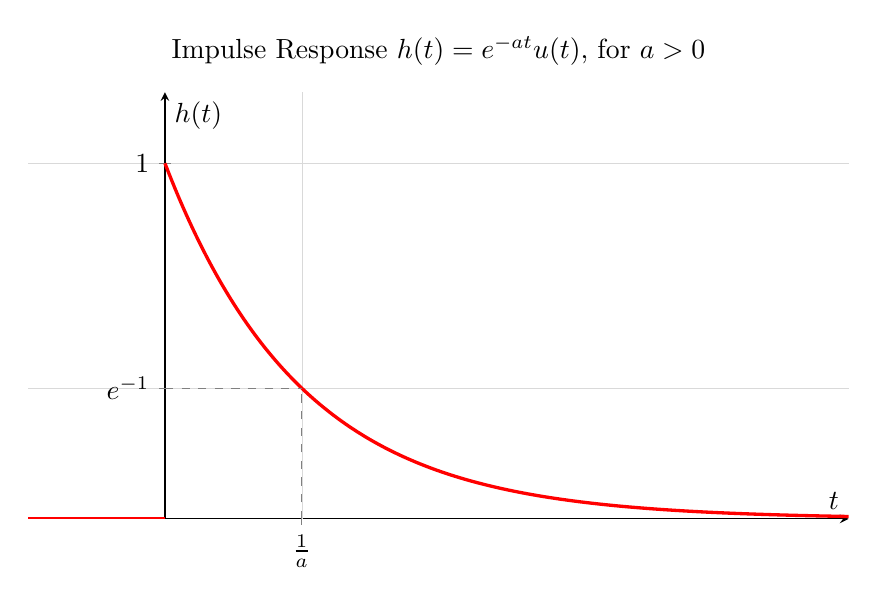
\begin{tikzpicture}
	\begin{axis}[
		width=12cm,
		height=7cm,
		title={Impulse Response $h(t) = e^{-at} u(t)$, for $a>0$},
		xlabel={$t$},
		ylabel={$h(t)$},
		axis lines=middle,
		xmin=-1, xmax=5,
		ymin=0, ymax=1.2,
		xtick=\empty,
		ytick=\empty,
		extra x ticks={1},
		extra x tick labels={$\frac{1}{a}$},
		extra y ticks={0.3678, 1},
		extra y tick labels={$e^{-1}$, $1$},
		grid=major,
		grid style={line width=.1pt, draw=gray!30},
		]
		
		% Plot the exponential decay for a=1
		\addplot[red, very thick, domain=0:5, samples=200, no marks] {exp(-x)};
		\draw[red, very thick] (axis cs:-1,0) -- (axis cs:0,0);
		
		% Add guidelines for the time constant
		\draw[dashed, gray] (axis cs:1,0) -- (axis cs:1, {exp(-1)});
		\draw[dashed, gray] (axis cs:0, {exp(-1)}) -- (axis cs:1, {exp(-1)});
		
	\end{axis}
\end{tikzpicture}}
        \caption{Impulse response $h(t) = e^{-at} u(t)$}
    \end{minipage}
\end{figure}

\textbf{Solution:}

$$y(t) = \int_{0}^{t} e^{-a(t-\tau)} d\tau = e^{-at} \int_{0}^{t} e^{a\tau} d\tau = \frac{1 - e^{-at}}{a}$$

For $t < 0$: $y(t) = 0$

\textbf{Answer:}
$$y(t) = \frac{1 - e^{-at}}{a} u(t)$$

\begin{figure}[H]
    \centering
    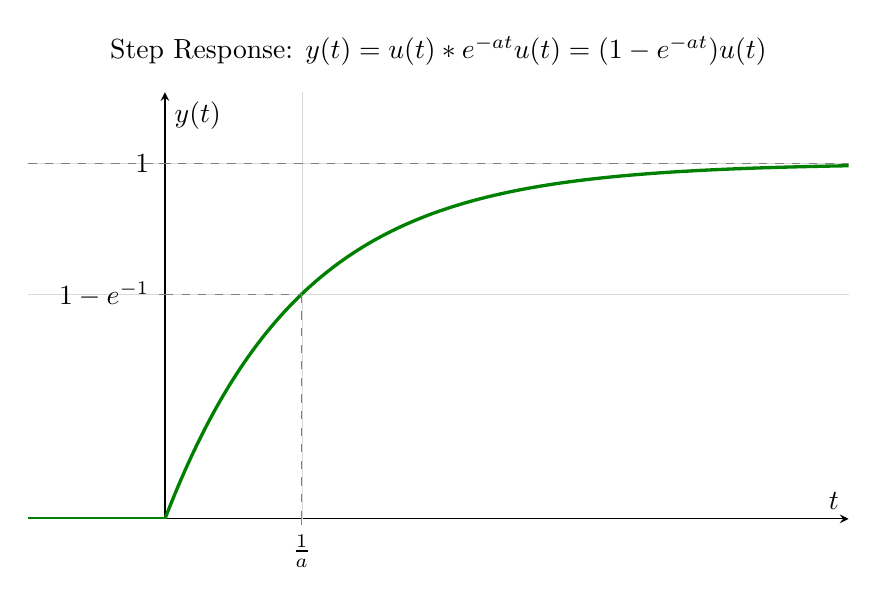
\begin{tikzpicture}
	\begin{axis}[
		width=12cm,
		height=7cm,
		title={Step Response: $y(t) = u(t) * e^{-at}u(t) = (1-e^{-at})u(t)$},
		xlabel={$t$},
		ylabel={$y(t)$},
		axis lines=middle,
		xmin=-1, xmax=5,
		ymin=0, ymax=1.2,
		xtick=\empty,
		ytick=\empty,
		extra x ticks={1},
		extra x tick labels={$\frac{1}{a}$},
		extra y ticks={0.632, 1},
		extra y tick labels={$1-e^{-1}$, $1$},
		grid=major,
		grid style={line width=.1pt, draw=gray!30},
		]
		
		% Plot the step response for a=1
		\addplot[green!50!black, very thick, domain=0:5, samples=200, no marks] {1 - exp(-x)};
		\draw[green!50!black, very thick] (axis cs:-1,0) -- (axis cs:0,0);
		
		% Plot the asymptote
		\addplot[dashed, gray, domain=-1:5] {1};
		
		% Add guidelines for the time constant
		\draw[dashed, gray] (axis cs:1,0) -- (axis cs:1, {1-exp(-1)});
		\draw[dashed, gray] (axis cs:0, {1-exp(-1)}) -- (axis cs:1, {1-exp(-1)});
		
	\end{axis}
\end{tikzpicture}
    \caption{Step response $y(t) = x(t) * h(t)$}
\end{figure}
\end{example}

\vspace{0.5em}
\hrule
\vspace{0.5em}

\begin{example}[2. Convolution of Two-Sided and One-Sided Signals]
\textbf{Problem:}
Find the convolution $y(t) = x(t) * h(t)$ where:
\begin{align}
    x(t) &= e^{-|t|} \quad \text{(two-sided exponential)} \\
    h(t) &= u(t) \quad \text{(unit step function)}
\end{align}

\begin{figure}[H]
    \centering
    \begin{minipage}{0.45\textwidth}
        \centering
        \resizebox{!}{5cm}{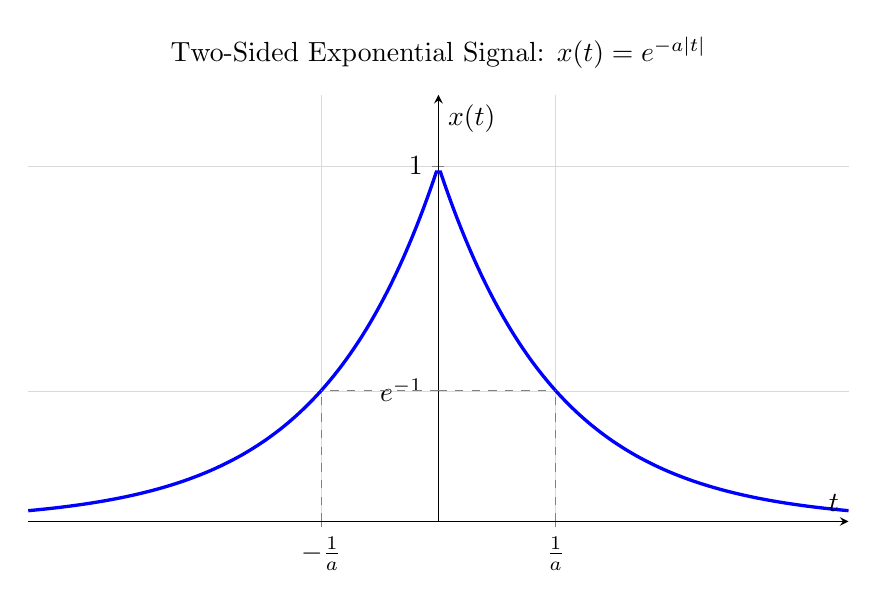
\begin{tikzpicture}
	\begin{axis}[
		width=12cm,
		height=7cm,
		title={Two-Sided Exponential Signal: $x(t) = e^{-a|t|}$},
		xlabel={$t$},
		ylabel={$x(t)$},
		axis lines=middle,
		xmin=-3.5, xmax=3.5,
		ymin=0, ymax=1.2,
		xtick={-1, 1},
		xticklabels={$-\frac{1}{a}$, $\frac{1}{a}$},
		ytick={0.3678, 1},
		yticklabels={$e^{-1}$, $1$},
		grid=major,
		grid style={line width=.1pt, draw=gray!30},
		]
		
		% Plot the function for a=1
		\addplot[blue, very thick, domain=-3.5:3.5, samples=200, no marks] {exp(-abs(x))};
		
		% Add guidelines
		\draw[dashed, gray] (axis cs:1,0) -- (axis cs:1, {exp(-1)});
		\draw[dashed, gray] (axis cs:-1,0) -- (axis cs:-1, {exp(-1)});
		\draw[dashed, gray] (axis cs:0,{exp(-1)}) -- (axis cs:1,{exp(-1)});
		\draw[dashed, gray] (axis cs:0,{exp(-1)}) -- (axis cs:-1,{exp(-1)});
		
	\end{axis}
\end{tikzpicture}}
        \caption{Input signal $x(t) = e^{-|t|}$}
    \end{minipage}\hfill
    \begin{minipage}{0.45\textwidth}
        \centering
       \resizebox{!}{5cm}{ \begin{tikzpicture}
	\begin{axis}[
		width=12cm,
		height=7cm,
		title={Impulse Response $h(t) = u(t)$},
		xlabel={$t$},
		ylabel={$h(t)$},
		axis lines=middle,
		xmin=-2.5, xmax=3.5,
		ymin=0, ymax=1.5,
		xtick={-2, -1, 1, 2, 3},
		ytick={1},
		grid=major,
		grid style={line width=.1pt, draw=gray!30},
		]
		
		% Draw the two parts of the function
		\draw[red, very thick] (axis cs:-2.5, 0) -- (axis cs:0, 0);
		\draw[red, very thick] (axis cs:0, 1) -- (axis cs:3.5, 1);
		
		% Mark the discontinuity at t=0
		\addplot[only marks, red, mark=*, mark size=2pt] coordinates {(0,1)};
		\addplot[only marks, red, mark=o, mark size=2pt, fill=white] coordinates {(0,0)};
		
	\end{axis}
\end{tikzpicture}}
        \caption{Impulse response $h(t) = u(t)$}
    \end{minipage}
\end{figure}

\textbf{Solution:}

$$y(t) = \int_{-\infty}^{t} e^{-|\tau|} d\tau$$

\textbf{Case 1:} $t < 0$
$$y(t) = \int_{-\infty}^{t} e^{\tau} d\tau = e^{t}$$

\textbf{Case 2:} $t \geq 0$
$$y(t) = \int_{-\infty}^{0} e^{\tau} d\tau + \int_{0}^{t} e^{-\tau} d\tau = 1 + (1 - e^{-t}) = 2 - e^{-t}$$

\textbf{Answer:}
$$y(t) = \begin{cases}
    e^{t} & \text{for } t < 0 \\
    2 - e^{-t} & \text{for } t \geq 0
\end{cases}$$

\begin{figure}[H]
    \centering
    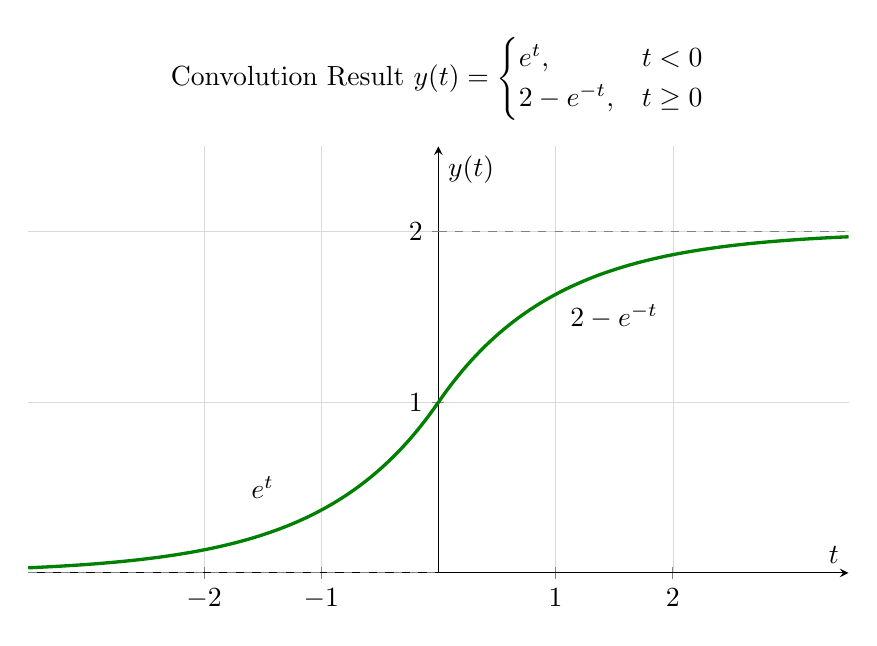
\begin{tikzpicture}
	\begin{axis}[
		width=12cm,
		height=7cm,
		title={Convolution Result $y(t) = 
			\begin{cases} 
				e^{t}, & t < 0 \\
				2-e^{-t}, & t \ge 0
			\end{cases}$
		},
		xlabel={$t$},
		ylabel={$y(t)$},
		axis lines=middle,
		xmin=-3.5, xmax=3.5,
		ymin=0, ymax=2.5,
		xtick={-2, -1, 1, 2},
		ytick={1, 2},
		grid=major,
		grid style={line width=.1pt, draw=gray!30},
		no marks,
		]
		
		% Plot the two parts of the function
		\addplot[green!50!black, very thick, domain=-3.5:0, samples=100] {exp(x)};
		\addplot[green!50!black, very thick, domain=0:3.5, samples=100] {2 - exp(-x)};
		
		% Plot the asymptotes
		\addplot[dashed, gray, domain=-3.5:0] {0};
		\addplot[dashed, gray, domain=0:3.5] {2};
		
		% Add labels for the function segments
		\node at (axis cs:-1.5, 0.5) {$e^{t}$};
		\node at (axis cs:1.5, 1.5) {$2-e^{-t}$};
		
	\end{axis}
\end{tikzpicture}
    \caption{Convolution result $y(t) = x(t) * h(t)$}
\end{figure}
\end{example}

\vspace{0.5em}
\hrule
\vspace{0.5em}

\begin{example}[3. Convolution with Rectangular Pulse]
\textbf{Problem:}
Find the convolution $y(t) = x(t) * h(t)$ where:
\begin{align}
    x(t) &= e^{-at} u(t), \quad a > 0 \\
    h(t) &= \begin{cases}
        1 & \text{for } 0 \leq t \leq T \\
        0 & \text{otherwise}
    \end{cases}
\end{align}

\begin{figure}[H]
    \centering
    \begin{minipage}{0.45\textwidth}
        \centering
         \resizebox{!}{5cm}{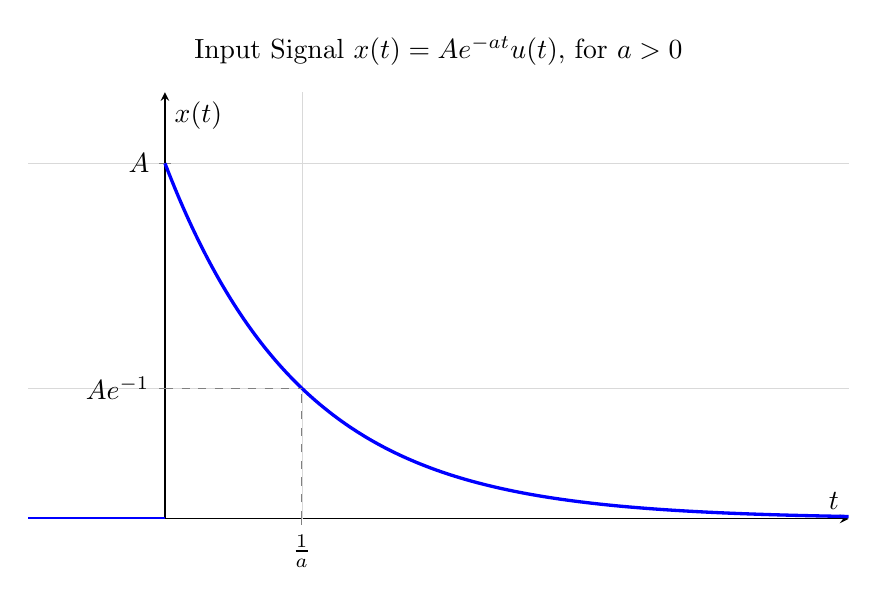
\begin{tikzpicture}
	\begin{axis}[
		width=12cm,
		height=7cm,
		title={Input Signal $x(t) = A e^{-at} u(t)$, for $a>0$},
		xlabel={$t$},
		ylabel={$x(t)$},
		axis lines=middle,
		xmin=-1, xmax=5,
		ymin=0, ymax=1.2,
		xtick=\empty,
		ytick=\empty,
		extra x ticks={1},
		extra x tick labels={$\frac{1}{a}$},
		extra y ticks={0.3678, 1},
		extra y tick labels={$Ae^{-1}$, $A$},
		grid=major,
		grid style={line width=.1pt, draw=gray!30},
		]
		
		% Plot the exponential decay for A=1, a=1
		\addplot[blue, very thick, domain=0:5, samples=200, no marks] {exp(-x)};
		\draw[blue, very thick] (axis cs:-1,0) -- (axis cs:0,0);
		
		% Add guidelines for the time constant
		\draw[dashed, gray] (axis cs:1,0) -- (axis cs:1, {exp(-1)});
		\draw[dashed, gray] (axis cs:0, {exp(-1)}) -- (axis cs:1, {exp(-1)});
		
	\end{axis}
\end{tikzpicture}}
        \caption{Input signal $x(t) = e^{-at} u(t)$}
    \end{minipage}\hfill
    \begin{minipage}{0.45\textwidth}
        \centering
        \resizebox{!}{5cm}{ \begin{tikzpicture}
	\begin{axis}[
		width=12cm,
		height=7cm,
		title={Rectangular Pulse $x(t) = u(t) - u(t-T)$},
		xlabel={$t$},
		ylabel={$x(t)$},
		axis lines=middle,
		xmin=-1, xmax=2.5,
		ymin=0, ymax=1.5,
		xtick={1},
		xticklabels={$T$},
		ytick={1},
		yticklabels={$A$},
		grid=major,
		grid style={line width=.1pt, draw=gray!30},
		]
		\draw[blue, very thick]
		(axis cs:-1,0) -- (axis cs:0,0) -- (axis cs:0,1) 
		-- (axis cs:1,1) -- (axis cs:1,0) -- (axis cs:2.5,0);
	\end{axis}
\end{tikzpicture}}
        \caption{Impulse response $h(t)$ (rectangular pulse)}
    \end{minipage}
\end{figure}

\textbf{Solution:}

$$y(t) = \int_{\max(0, t-T)}^{t} e^{-a\tau} d\tau$$

\textbf{Case 1:} $t < 0$ → $y(t) = 0$

\textbf{Case 2:} $0 \leq t \leq T$
$$y(t) = \int_{0}^{t} e^{-a\tau} d\tau = \frac{1 - e^{-at}}{a}$$

\textbf{Case 3:} $t > T$
$$y(t) = \int_{t-T}^{t} e^{-a\tau} d\tau = \frac{e^{-a(t-T)} - e^{-at}}{a} = \frac{e^{-at}(e^{aT} - 1)}{a}$$

\textbf{Answer:}
$$y(t) = \begin{cases}
    0 & \text{for } t < 0 \\
    \frac{1 - e^{-at}}{a} & \text{for } 0 \leq t \leq T \\
    \frac{e^{-at}(e^{aT} - 1)}{a} & \text{for } t > T
\end{cases}$$

\begin{figure}[H]
    \centering
    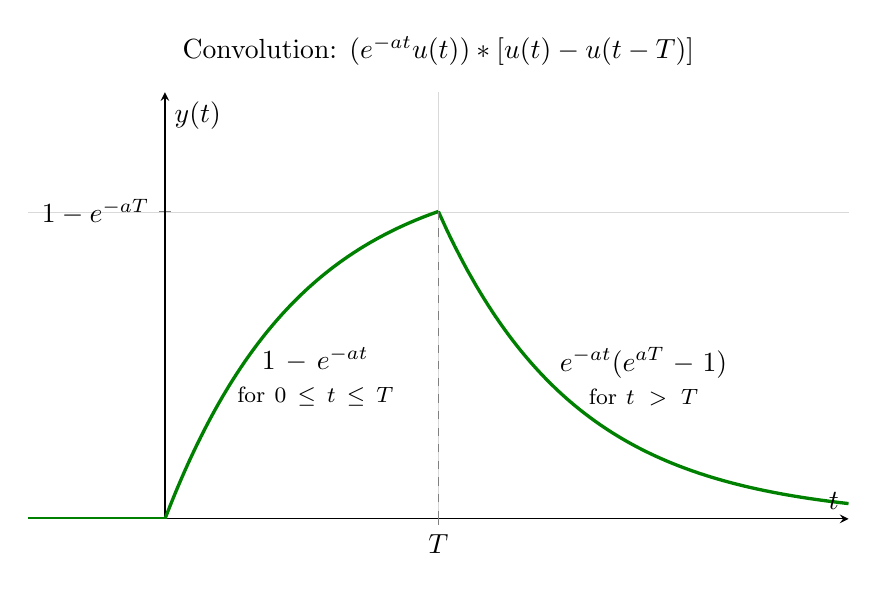
\begin{tikzpicture}
	\begin{axis}[
		width=12cm,
		height=7cm,
		title={Convolution: $(e^{-at}u(t)) * [u(t)-u(t-T)]$},
		xlabel={$t$},
		ylabel={$y(t)$},
		axis lines=middle,
		xmin=-1, xmax=5,
		ymin=0, ymax=1.2,
		xtick={2},
		xticklabels={$T$},
		ytick={0.864},
		yticklabels={$1-e^{-aT}$},
		grid=major,
		grid style={line width=.1pt, draw=gray!30},
		no marks,
		]
		
		% Plot the two parts of the convolution result for a=1, T=2
		\addplot[green!50!black, very thick, domain=0:2, samples=100] {1 - exp(-x)};
		\addplot[green!50!black, very thick, domain=2:5, samples=100] {exp(-x)*(exp(2)-1)};
		\draw[green!50!black, very thick] (axis cs:-1,0) -- (axis cs:0,0);
		
		% Add vertical line at t=T
		\draw[dashed, gray] (axis cs:2,0) -- (axis cs:2, {1-exp(-2)});
		
		% Add labels for the function segments
		\node[text width=3cm, align=center] at (axis cs:1.1, 0.4) {$1-e^{-at}$ \\ \footnotesize for $0 \le t \le T$};
		\node[text width=3cm, align=center] at (axis cs:3.5, 0.4) {$e^{-at}(e^{aT}-1)$ \\ \footnotesize for $t > T$};
		
	\end{axis}
\end{tikzpicture}
    \caption{Convolution result $y(t) = x(t) * h(t)$}
\end{figure}
\end{example}

\vspace{0.5em}
\hrule
\vspace{0.5em}

\begin{example}[4. Convolution with Impulse Train]
\textbf{Problem:}
Find $y(t) = x(t) * h(t)$ where $x(t) = \cos(\omega_0 t)$ and $h(t) = \sum_{n=-\infty}^{\infty} \delta(t - nT)$.

\textbf{Solution:}
Using sifting property: $y(t) = \sum_{n=-\infty}^{\infty} \cos(\omega_0 (t - nT))$

Using the identity $\cos(A-B) = \cos A \cos B + \sin A \sin B$:
$$y(t) = \sum_{n=-\infty}^{\infty} [\cos(\omega_0 t)\cos(\omega_0 nT) + \sin(\omega_0 t)\sin(\omega_0 nT)]$$

$$= \cos(\omega_0 t) \sum_{n=-\infty}^{\infty} \cos(\omega_0 nT) + \sin(\omega_0 t) \sum_{n=-\infty}^{\infty} \sin(\omega_0 nT)$$

Since $\sum_{n=-\infty}^{\infty} \sin(\omega_0 nT) = 0$ (odd symmetry):
$$y(t) = \cos(\omega_0 t) \sum_{n=-\infty}^{\infty} \cos(\omega_0 nT)$$

\textbf{Answer:} $y(t) = \cos(\omega_0 t) \sum_{n=-\infty}^{\infty} \cos(\omega_0 nT)$
\end{example}

\end{document}